\section{Sprawdzanie poprawności schematu}
\label{sec:sprawdzanie_poprawnosci_schematu}

Dla każdego poziomu wymagania zapisane są w SO \texttt{Level}, który opisuje,
jakiego rodzaju wymagany jest tranzystor,
między jakimi węzłami powinien się znajdować,
a także jakie są wymagane wymiary bramki.
Przykładowe wymagania dla poziomu 1 przedstawiono na rys.~\ref{fig:level1_requirements}.

\begin{figure}[h]
    \centering
    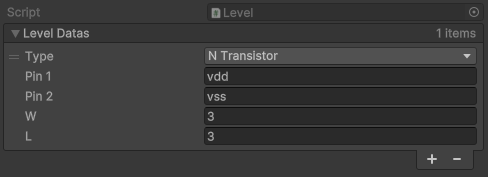
\includegraphics[width=.9\textwidth]{chapters/chapter4/rys/level}
    \caption[Przykładowe wymagania dla poziomu 1.]
    {Przykładowe wymagania dla poziomu 1, źródło: opracowanie własne.}
    \label{fig:level1_requirements}
\end{figure}

Za sprawdzanie poprawności schematu odpowiada komponent \texttt{CheckerManager}, dziedziczący po \texttt{MonoSingleton}.
Zadaniem tego komponentu jest wywołanie skryptu walidującego narysowany schemat,
a następnie porównanie wyników z wymaganiami poziomu.
Na tej podstawie decyduje, czy schemat jest poprawny, czy też nie\linebreak
i wywołuje okno wyników, które informuje użytkownika o rezultacie.

\subsection{Walidacja schematu}
\label{subsec:walidacja_schematu}

Walidacją schematu zajmuje się komponent \texttt{TopographyValidator}.
Po wywołaniu startu walidacji przez \texttt{CheckerManager},
w pierwszej kolejności wyszukiwane są oznaczenia węzłów, $V_{SS}$ i $V_{DD}$.
Są one punktami zaczepienia dla schematu, a ich brak oznacza błąd.
Gdy znaleziono oba węzły, pobierana jest komórka, jaka znajduje się pod węzłem $V_{DD}$,
przy wykorzystaniu \texttt{Physics.Raycast}.
Komórka ta pełni funkcję punktu startowego w algorytmie znajdywania połączeń.\\
\indent W pierwszej kolejności lokalizowane są wszystkie tranzystory na schemacie.
W tym celu z \texttt{LayersManager} pobierane są wszystkie komórki z warstwy \textit{Poly Crystal}.
Dla każdej z komórek sprawdzane jest, 
czy znajduje się pod nią komórka z warstwy \textit{N Diffusion} lub \textit{P Diffusion}.
Do tego celu wykorzystywana jest kolejna funkcja z zasobu systemu fizyki Unity, \texttt{Physics.OverlapBox},
wykrywa ona obiekty znajdujące się wewnątrz lub stykające z zadanym obszarem.
Jeśli udało się wykryć komórkę z warstw dyfuzyjnych, to znaczy, że znaleziono część tranzystora.
%Tworzony jest wtedy nowy obiekt dziedziczący po klasie \texttt{Transistor}, \textt{NTransistor} lub \texttt{PTransistor},
%odpowiednio dla tranzystorów nMOS lub pMOS.
Tworzony jest wtedy nowy obiekt dziedziczący po klasie \texttt{Transistor}:
\texttt{NTransistor} dla tranzystorów nMOS lub \texttt{PTransistor} dla tranzystorów pMOS.
W konstruktorze natomiast przekazywane są już znalezione komórki warstwy polikrystalicznej i dyfuzyjnej.
Obiekt ten ma na celu przechowywanie informacji o tranzystorze oraz wykrycie własnych parametrów.
Po jego utworzeniu wywoływana jest w nim metoda \texttt{FindRest}.
Na podstawie przekazanych wcześniej komórek, ponownie stosując \texttt{Physics.OverlapBox},
znajdywane są sąsiadujące komórki warstw dyfuzyjnej i polikrystalicznej, które się na siebie nakładają.
Aby znaleźć wszystkie komórki, które należą do tranzystora, wykorzystywana jest rekurencja
-- każda znaleziona komórka również próbuje znaleźć sąsiadujące z nią komórki.
Aby uniknąć ponownego wykrycia, komórki po znalezieniu są wyłączane,
dzięki czemu \texttt{Physics.OverlapBox} ich nie wykryje.
Po wyśledzeniu wszystkich komórek, które należą do tranzystora,
w ich miejsce wstawiany jest pojedynczy GO z \texttt{BoxCollider}'em,
do których referencje są przechowywane w obiekcie tranzystora.
Dzięki temu znacząco uproszczone będzie wykrycie połączeń.
Przy ustawianiu rozmiaru komponentu \texttt{BoxCollider}, przy okazji obliczane są wymiary bramki tranzystora,
Główny kod funkcji do znajdywania tranzystorów przedstawiona jest na listingu~\ref{lst:find_transistors}.
Aby uniknąć zawieszenia się pętli programu,
zastosowano przy wyszukiwaniu komórek tranzystora system asynchroniczności \textit{UniTask}.
\newpage

\begin{lstlisting}[language={C},label=lst:find_transistors,caption={Metoda \texttt{FindTransistors} wyszukjąca tranzystory na schemacie}]
private async UniTask FindTransistors() {
    var polys = LayersManager.Instance.LayerHolders[polyLayer].Cells;
    List<GameObject> usedPolys = new();
    Vector3 overlapSize = new Vector3(0.45f, 0.45f, 0.6f);
    foreach (var poly in polys) {
        if (usedPolys.Contains(poly)) continue;
        var position = poly.transform.position;
        position.x += 0.5f;
        position.y += 0.5f;
        position.z += 0.5f;
        var overlaps = Physics.OverlapBox(position, overlapSize);
        foreach (var overlap in overlaps) {
            if (overlap.gameObject.CompareTag("P Diffusion")) {
                var pTransistor = new PTransistor(poly, overlap.gameObject); 
                await pTransistor.FindRest();
                pTransistor.CreateCollider().Forget();
                usedPolys.AddRange(pTransistor.Polys);
                _pTransistors.Add(pTransistor);
            }
            else if (overlap.gameObject.CompareTag("N Diffusion")) {
                var nTransistor = new NTransistor(poly, overlap.gameObject);
                await nTransistor.FindRest();
                nTransistor.CreateCollider().Forget();
                usedPolys.AddRange(nTransistor.Polys);
                _nTransistors.Add(nTransistor);
            }
        }
    }
    await UniTask.Yield();
    await UniTask.Yield();
}

\end{lstlisting}

Po znalezieniu wszystkich tranzystorów wywoływana jest funkcja \texttt{StartSearch}.
Rozpoczyna ona przeszukiwanie połączeń od komórki pod oznaczeniem $V_{DD}$.\linebreak
W pierwszej kolejności tworzony jest obiekt węzła \texttt{Node}, oznaczony jako \textit{vdd},
który przechowuje w listach wszystkie znalezione komórki,
kontakty oraz tranzystory typu p i n.
Następnie wywoływana jest metoda \texttt{SearchByOverlap},
której przekazywana jest pozycja startowej komórki oraz obecny węzeł.
Ma ona za zadanie znaleźć wszystkie obiekty sąsiadujące z obecnym,
na podstawie \texttt{Physics.OverlapBox}.
i zapisanie ich do odpowiednich list w obiekcie \texttt{Node}.\\
\indent Jeśli znaleziono tranzystor, należy połączyć go z węzłem,
co jest wykonywane przez funkcję \texttt{ConnectTransistor}.
Obiekt \texttt{Transistor} przypisuje do wolnego pinu obecny węzeł,
zapisując także, po jakiej stronie tranzystora znajduje się ten pin,
jak również to, że drugi wolny pin jest po przeciwnej stronie.\\
\indent Gdy znalezionym obiektem w funkcji \texttt{SearchByOverlap} jest komórka,
dla niej również wywoływana jest ta funkcja. %, a jako \texttt{Node} przekazywany jest ten obecnie przeszukiwany.
Aby uniknąć ponownego wykrywania, podobnie jak w przypadku tranzystorów,
już znalezione komórki są wyłączane.\\
\indent Po zidentyfikowaniu wszystkich obiektów dla danej warstwy,
jeśli znaleziono kontakty, ponawia się przeszukiwanie, dla tej warstwy, z którą występuje połączenie.
Natomiast dla każdego ze znalezionych tranzystorów,
tworzony jest nowy węzeł po stronie wolnego pinu tranzystora,
do którego jest też automatycznie podłączany.
%Następnie całość procesu jest powtarzana dla nowego węzła, tak jak dla węzła \textit{vdd}.
Następnie cały proces, jaki miał miejsce dla \textit{vdd}, zostaje powtórzony dla nowego węzła.
Dla każdej badanej pozycji jest także dodatkowo sprawdzane, czy nie pokrywa się z oznaczeniem $V_{SS}$.
Jeśli tak, to obecny węzeł jest oznaczany jako \textit{vss}.
Proces znajdywania połączeń jest powtarzany, aż do momentu,
gdy nie będzie już możliwe wykrycie nowych obiektów.
Główną funkcję \texttt{SearchByOverlap} odpowiedzialną za przeszukiwanie przedstawiono na listingu~\ref{lst:search_overlap}.
Ponownie zastosowano tutaj system asynchroniczności \textit{UniTask}.

\begin{lstlisting}[language={C},label=lst:search_overlap,caption={Metoda \texttt{SearchOverlap} wykrywające sąsiadujące obiekty}]
private async UniTask SearchByOverlap(Vector3 center, Node node) {
    center.x += 0.5f;
    center.y += 0.5f;
    var overlaps = Physics.OverlapBox(center, _overlapSize);
    foreach (var overlap in overlaps) {
        if (CheckForVss(overlap.transform.position)) node.ChangeID("vss");
        if (overlap.gameObject.CompareTag("Contact"))  {
            if (node.Contacts.Contains(overlap.gameObject)) continue;
            node.Contacts.Add(overlap.gameObject);
            overlap.gameObject.SetActive(false);
        }
        else if (overlap.gameObject.CompareTag("P Transistor")) {
            var pTransistor = FindPTransistor(overlap.gameObject);
            if (node.PTransistors.Contains(pTransistor)) continue;
            ConnectTransistor(node, pTransistor, overlap.transform.position);
        }
        else if (overlap.gameObject.CompareTag("N Transistor")) {
            var nTransistor = FindNTransistor(overlap.gameObject);
            if (node.NTransistors.Contains(nTransistor)) continue;
            ConnectTransistor(node, nTransistor, overlap.transform.position);
        }
        else {
            var position = overlap.transform.position;
            node.Cells.Add(overlap.gameObject);
            overlap.gameObject.SetActive(false);
            await SearchByOverlap(position, node);
        }
    }
}

\end{lstlisting}

\subsection{Finalizacja sprawdzania}
\label{subsec:finalizacja_sprawdzania}

Po zakończeniu walidacji przez \texttt{TopographyValidator} wywołuje on wydarzenie \texttt{OnValidationEnd},
w którym przekazuje wszystkie wykryte tranzystory, wraz z ich połączeniami i wymiarami.
Iterując po elementach zawartych w wymaganiach poziomu,
porównuje się je z wykrytymi tranzystorami.
Gdy któryś z tranzystorów spełnia jedno z wymagań, jest usuwany z listy wykrytych.
Jeśli pod koniec w liście wykrytych tranzystorów nie ma już żadnych elementów,
oznacza to, że schemat jest poprawny.
Wyświetlane jest wtedy okno informujące o sukcesie.
W przeciwnym wypadku gdy pozostały jeszcze tranzystory, to znaczy, że schemat jest niepoprawny.